
\subsection{Depth Sensor Based Reconstruction}

In this section we describe the process of projecting, registering and integrating 3D reconstructions from depth sensor based input. Depth Sensor based input is fast and reliable but such date not only requires specialized hardware, it also has several draw-backs discussed here. One drawback is that accuracy is limited by the resolution of the device. This means if the application requires higher resolution (more than the standard $640\times 480$) another technique (possibly based on stereo cameras of higher resolution may be required). Another drawback is that certain materials reflect infra-red light, meaning their depth/structure cannot be computed. Salient points within an image typically occur at the edges and corners of objects, these locations however, are known to produce noisy depth information at these pixel locations. \\

A major reason to choose depth sensor based reconstruction frameworks is the consistency and speed of depth data input. For scenes which are easily scanned by depth sensors, this sensor type is typically a preferred choice. A useful sensor input for 3D Fourier Volume Registration includes a color and depth image pair, $f(u,v)$ and $g(u,v)$ respectively. In our experiments, these are obtained using an Asus Xtion PRO LIVE sensor such that $u \in \{0..639\}$ and $v \in \{0..479\}$. Examples of these images are shown in figures \ref{fig:COLEXAMPLE} and \ref{fig:DEPTHEXAMPLE}. Using $Z_{u,v}$ = $g(u,v)$, $f(u,v)$ is projected into 3D space using equation \ref{eqn:PC_PROJECTION} to obtain the $X_{u,v}$ and $Y_{u,v}$ coordinate values in 3D space. Here, $c_x$ and $c_y$ represent the intersection point where the optical axis intersects the projection plane and are defined as $c_x = 319.5$, $c_y = 239.5$. Also $f_x$ and $f_y$ represent the focal length which is defined as $f_x$, $f_y = 525.0$. \\


\begin{equation} \label{eqn:PC_PROJECTION}
\begin{split}
X_{u,v} & = \frac{(u - c_x)Z_{u,v}}{f_x} \\
Y_{u,v} & = \frac{(v - c_y)Z_{u,v}}{f_y} \\
\end{split}
\end{equation}

\begin{figure}[t!] 
        \centering
        \begin{subfigure}[b]{1.8in}
                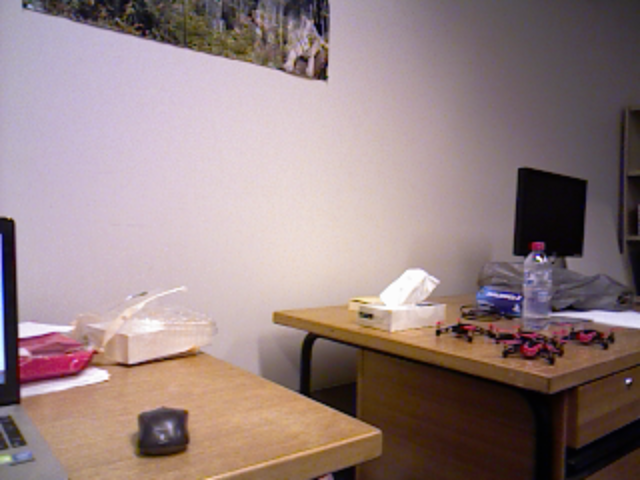
\includegraphics[width=1.7in]{images/ch2/colorF11}
                \caption{Color Image}
                \label{fig:COLEXAMPLE}
        \end{subfigure}%
        \begin{subfigure}[b]{1.8in}
                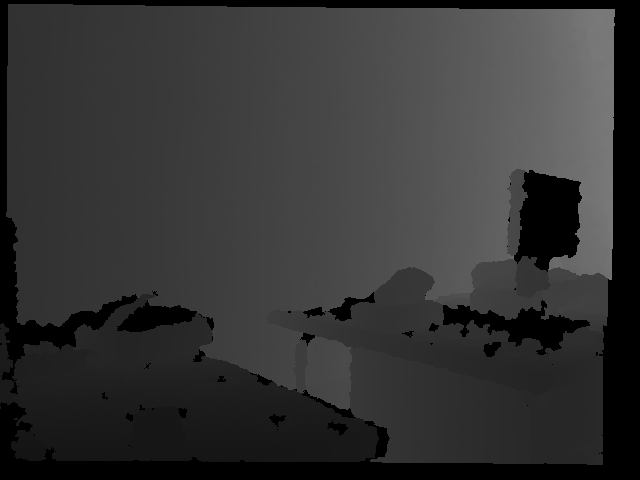
\includegraphics[width=1.7in]{images/ch2/depthF11}
                \caption{Depth Image}
                \label{fig:DEPTHEXAMPLE}
        \end{subfigure}
        
         \begin{subfigure}[b]{1.8in}
                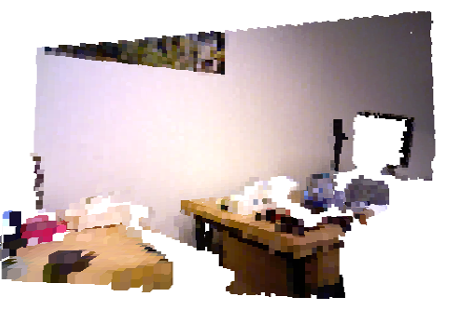
\includegraphics[width=1.8in]{images/ch2/volumeF11128}
                \caption{Projected Volume $128^3$}
                \label{fig:VOLUMEEXAMPLE128}
        \end{subfigure}%
         \begin{subfigure}[b]{1.8in}
                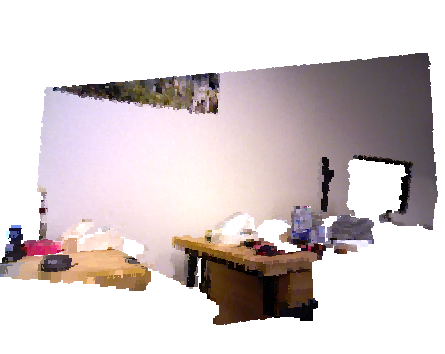
\includegraphics[width=1.8in]{images/ch2/volumeF11256}
                \caption{Projected Volume $256^3$}
                \label{fig:VOLUMEEXAMPLE384}
        \end{subfigure}%
       \caption{A Projected Frame.}
       \label{fig:PROJECTED_FRAME}
\end{figure}


To facilitate further processing, the projected image volumes are re-sampled. The results reported in this paper were obtained using volumes of $256^3$ voxels in size. An example colour and depth image pair and their volumetric projection is shown in figure \ref{fig:PROJECTED_FRAME}.  \\


\subsection{Stereo Camera Based Reconstruction}

The Fourier volume registration methods also work with stereo camera based data. This information can be generated using several of the techniques described in the literature review. Essentially the data must then be projected into depth frames which are registered using one of the proposed fourier volume registration techniques. Because stereo methods do not always accurately compute depth to scale, fourier volume registration has an advantage over other methods in that it also registers against scale. For systems where depth is estimated accurately (as accurately or more than depth sensors) results should work similarly.

\subsection{Monocular Sensor Based 3D Reconstruction}

Some preliminary research has been conducted in evaluating the use of Fourier volume registration given monocular data. From monocular video frames, depth was first computed. This data was fed into the fourier volume registration method in computing 3D reconstructions. Preliminary results are presented but further investigation is required in this area.

